\documentclass{article}
\usepackage{graphicx}
\usepackage{float} 
\usepackage{amsmath, amssymb, amsthm}
\usepackage{tcolorbox}
\usepackage{hyperref}
\graphicspath{{images/}}
\usepackage[letterpaper, top=1.0in, bottom=1.0in, left=1.0in, right=1.0in, heightrounded]{geometry}
\usepackage{url}
\renewcommand{\baselinestretch}{1.50}
\setlength{\parindent}{0pt}
\setlength{\parskip}{0.8em}

\title{RSA Encryption in Theory and Practice}
\author{Paige Haines}
\date{September 2024}

\begin{document}

\maketitle
\begin{abstract}
    This report explores the mathematical fundamentals of the RSA cryptosystem, the theorems and definitions that support it, and its application in modern day. We begin with exploring RSA key generation, encryption and decryption, using examples and detailed proofs to demonstrate each step of the process. Concepts such as Euler's theorem, and totient function, modular inverses and successive squaring are discussed to emphasise their roles in the RSA algorithm. We conclude by analysing its vulnerabilities, including potential weaknesses such as the looming threat of quantum computing. Additionally, we discuss its practical applications in cryptography and its role in ensuring secure communication in our day-to-day.
\end{abstract}

\section{Introduction}
Since its inception in $1977$ by renowned cryptographers Ron Rivest, Adi Shamir and Leonard Adleman \cite{rsa1977}, the RSA encryption algorithm is a public-key cryptosystem that ensures secure data transmission over networks. Its security is supported by the principles of number theory, and the sheer difficulty of prime factorisation of large numbers.  Relying on concepts such as modular arithmetic and prime factorisation to perform its encryption and decryption processes, confidentiality, integrity, and authenticity are maintained when communicating digitally. In response to the implications of symmetric key cryptography, RSA was developed to provide a more secure method of exchanging keys. In a public-key encryption cryptosystem, a public encryption key is revealed, yet this doesn't compromise the decryption private key. This development had a significant impact on the future of secure communication online. In this paper, a detailed exploration of the RSA algorithm will be illustrated, highlighting its definition, and mathematical principles such as modular exponentiation, prime factorisation and Euler's theorem to analyse the strength of the RSA encryption algorithm. This exploration includes practical applications of this algorithm and its implications in practice. 

\begin{enumerate}
    \item Apply the decryption procedure on an enciphered message yields the original message, $M$. Formally:
\begin{equation}
    D(E(M)) \equiv M
\end{equation}
    \item Both encryption procedures and decryption procedures are easy to compute.
    \item Despite publicly revealing $E$, there is no easy way to compute $D$.
    \item If a given message $M$ is first deciphered utilising decryption procedure $D$ and then subsequently enciphered utilising encryption procedure $E$, the original message $M$ remains the result: 
\begin{equation}
        E(D(M)) \equiv M
\end{equation}
\end{enumerate}
While intuitive, this algorithm had its shortfalls, most notably its susceptibility to man-in-the-middle attacks and lack of authenticity, which ultimately led to the introduction of the RSA cryptosystem.

\section{Mathematical Foundations of the RSA Algorithm}
The RSA algorithm adopts many components of discrete mathematics including modular arithmetic, prime factorisation, and Euler's totient function. Modular arithmetic is utilised in the key generation and encryption process of the algorithm, coupled with functions such as Euler's totient function. The preceding sections will detail definitions of important mathematical concepts which form the basis of the RSA algorithm.

\subsection{Definitions}
\subsubsection{Modular Arithmetic}
Defined as an arithmetic system of integers, modular arithmetic explores the concept of numbers wrapping around when they reach a predetermined integer –the modulus. For a positive integer $n$, integers $a$ and $b$ are congruent $\mod n$ if they share the same remainder when divided by $n$:
\begin{equation}
a \equiv b \mod n
\end{equation}
If $b$ divides $a$ if there exists some integer $k$ such that 
\begin{equation}
a = b + kn
\end{equation}
This signifies that $a$ and $b$ have the same remainder when divided by $n$ as they share a common factor $k$. 

In RSA, both the encryption and decryption processes involve exponentiation and taking results modulo a large integer . In modular arithmetic, computations are able to be managed and prevent the size of the numbers from growing excessively large.

\subsubsection{Prime Numbers}
We define a prime number as a natural number greater than $1$ that has no other positive divisors other than $1$ and itself. We formally state that an integer $p$ is prime if $p > 1$ and for any integer $d$ that divides $p$, $d$ will be either $p$ or $1$. Prime numbers provide a unique property to the RSA algorithm due to their divisibility qualities and difficulty to factor. 

In RSA, prime numbers $p$ and $q$ are selected to create a large modulus $n = pq$. Factoring $n$ into its prime factors is computationally difficult and this fact forms the basis of RSA’s security. While it is easy to multiply two primes, reversing the multiplication process of $p$ and $q$ is not.

\subsubsection{Euler's Totient Function}
Euler's totient function denoted as $\phi$ is defined by the following integer mapping:
\begin{equation}
\phi: \mathbb{Z} \to \mathbb{Z}
\end{equation}

This means that the function takes an integer $n \in \mathbb{Z}$ and maps it to another integer $\phi(n) \in \mathbb{Z}$. In other words, it counts the number of integers $a$ that are $\leq n$ that are relatively prime to $n$ meaning $gcd(a,n) = 1$ for $1 \leq a \leq n$. Euler's totient function can be broken down into two distinct cases:
\begin{enumerate}
    \item If $n$ is prime: $\phi(n) = n-1$, because all integers less than $n$ are relatively prime to $n$.
    \item If $n$ is a product of two positive prime integers $p$ and $q$, then the function evaluates:
\begin{equation}
\phi(n) = (p-1)(q-1)
\end{equation}
\end{enumerate}
The value derived from Euler's totient function, $\phi(n)$, is used in computing the modular inverse using Euler's theorem which states $a^{\phi(n)} \equiv 1 \mod n$ when $gcd(a,n) = 1$. This problem is simplified to exponentiation $\mod n$. As RSA deals with large prime integers, Euler's totient allows for efficient calculation when combined with modular exponentiation. 

\subsubsection{Modulus $n$, Public Key $\{n, e\}$, and Private Key $\{n, d\}$}
There are three key components that the RSA algorithm is comprised of that give it its functionality. As the RSA algorithm utilised two different key procedures for encryption and decryption, the security of the RSA algorithm relies on the use of these components. 

\textbf{Modulus $n$} refers to the product of two large prime integers $p$ and $q$, denoted $n = pq$ and this modulus is used in the public and private keys of the algorithm. 

\textbf{Public key}$\{n, e\}$ is comprised of the modulus $n$ and a public exponent $e$, which is typically a small prime number that is used to encrypt messages and satisfies the condition $gcd(e, \phi(n)) = 1$. 

\textbf{Private key}$\{n, d\}$ consists of the modulus $n$ and a private exponent $d$, which is the modular inverse of $e \mod \phi (n)$ and satisfies the condition $e \cdot d = 1 \mod \phi(n)$. This is the decryption key.

\subsubsection{Greatest Common Divisor}
The greatest common divisor between two integers (denoted $gcd(a, b)$) is the largest integer that divides both $a$ and $b$ without leaving a remainder such that $d | a$, and $d | b$. When selecting a public exponent $e$, we must ensure that $e$ is relatively prime to $\phi(n)$, meaning that $gcd(e, \phi(n)) = 1$. This formula ensures that there exists a multiplicative inverse for $e\mod \phi (n)$, which is necessary for computing the private exponent $d$. 

\subsection{Key Concepts}
Two concepts are applied to ensure the efficiency of the RSA algorithm – Euler's Theorem \cite{eulerstheorem} and Modular Inverses.

\begin{tcolorbox}[colback=orange!5!white, colframe=orange!50!white, title=\textbf{Theorem 2.1 (Euler)}]
If $a$ and $n$ are relatively prime positive integers, then 
\begin{equation}
a^{\phi(n)} \equiv 1 \mod n
\end{equation}
where $\phi(n)$ counts every positive integer up to $n$ that is relatively prime to $n$. 
\end{tcolorbox}
\begin{proof}
    Let $n$ be a positive integer, and $a$ an integer such that $gcd(a, n) = 1$. We aim to show that $a^{\phi(n)} \equiv 1 \mod n$. We begin by defining a set of integers that are relatively prime to $n$: 
\begin{equation}
S = \{ u_1, u_2, u_3, \ldots, u_{\phi(n)} \}
\end{equation}
where each $u_1$ is a distinct positive integer satisfying $1 \leq u_i \leq n$ and $gcd(u_i, n) = 1$. We now consider the set that is formed by multiplying each element of set $S$ by $a$:
\begin{equation}
aS = \{ au_1, au_2, \ldots, au_{\phi(n)} \}
\end{equation}
Since $gcd(a, n) = 1$, a has a multiplicative inverse $\mod n$ multiplying each element in $S$ by $a$ permutes the elements of $S$, meaning that $aS$ contains all distinct elements $\mod n$. To further illustrate, for any element $b \in S$, the equation
\begin{equation}
ax \equiv b \mod n
\end{equation}
is able to be solved as $a$ has a multiplicative inverse $\mod n$. This means for every $b$, we are able to find an $x$ such that we can establish a connection between $b$ and a corresponding $au_i$. Comparing the elements in both sets $S$ and $aS$:
\begin{equation}
u_1u_2 \ldots u_{\phi(n)} \equiv (au_1)(au_2) \ldots (au_{\phi(n)}) \mod n
\end{equation}
We can expand and subsequently refactor this equation as follows:
\begin{equation}
u_1u_2 \ldots u_{\phi(n)} \equiv a^{\phi(n)}u_1u_2 \ldots u_{\phi(n)} \mod n
\end{equation}
As each $u_i$ is relatively prime to $n$, this product $u_1u_2u_3 \ldots u_{\phi(n)} \ncong 0 \mod n$ means we are able to divide on both sides by this product yielding
\begin{equation}
1 \equiv a^{\phi(n)} \mod n
\end{equation}
We have concluded that $ a^{\phi(n)} \mod n \equiv 1$, thus completing the proof.
\end{proof}

The proof outlined above demonstrates a key idea – that multiplying the set $S$ of integers relatively prime to $n$ permutes the original set ($gcd(a, n) = 1$), and set $aS$ contains the exact same elements as set $S$, simply in a different order. This very relationship highlights the congruence between set $S$ and $aS$. By expanding the product of $aS$ to $a^{\phi(n)}\cdot u_1u_2 \ldots u_{\phi(n)}$ and the product $u_1u_2 \ldots u_{\phi(n)} \mod n \ncong 0$, we divide on both sides by the product, leaving the result $1 \equiv a^{\phi(n)} \mod n$. This occurs because $a$ has an inverse $\mod n$ such that $S$ and $aS$  $\equiv \mod n$. 

Euler's theorem and its properties provide the foundation for the decryption process of the RSA algorithm, as it provides a means of implementing modular exponentiation, which allows the exponentiation by $d$ to reverse the encryption by $e$, guaranteeing correctness of the algorithm.
\begin{tcolorbox} [colback=purple!5!white, colframe=purple!40!white, title=\textbf{Definition (Modular Inverse)}]
Integer $a$ has a modular inverse modulo $n$ if and only if $a$ and $n$ are relatively prime and such that their greatest common divisor is $1$: $gcd(a, n) = 1$. We define the modular inverse of an integer $a$ as an integer $x$ such that
\begin{equation}
a \cdot x \equiv 1 \mod n
\end{equation}
holds true such that when $a \cdot x$ is divided by $n$, the result is 1.    
\end{tcolorbox}

\begin{tcolorbox} [colback=gray!5!white, colframe=gray!40!white, title=\textbf{Corollary 2.2.1 (Bézout's Lemma)}]
Given two integers $a$ and $n$, if $gcd(a, n) = 1$, there exist two integers $x$ and $y$ such that $a \cdot x + n \cdot y = 1$ where $x$ is the modular inverse of $a \mod n$. 
\end{tcolorbox}

Bézout's lemma presents the conditions for which a modular inverse exists – when $a$ and $n$ are relatively prime.

The modular inverse aids in the generation of the private exponent $d$, as when given the public exponent $e$ and Euler's totient function $\phi(n)$, the private exponent $d$ is identified as the modular inverse of $e \mod \phi(n)$ such that
\begin{equation}
e \cdot d \equiv 1 \mod \phi(n)
\end{equation}
This connection ensures that raising the ciphertext $C$ to the power of $d$ reverses the encryption process performed by $C = M^e \mod n$ where $M$ is our original message. We can show the existence of this modular inverse as $e$ and $\phi(n)$ are relatively prime, through our proof of Euler's theorem and $gcd(e, \phi(n)) = 1$.

\subsection{RSA Key Generation}
RSA key generation is the process in which two cryptographic keys are created – public key $e$, and private key $d$ for use in secure communication. As the name suggests, public key $e$ is shared with others and is utilised to encrypt messages. Private key $d$ is kept strictly confidential and is used to decrypt messages encrypted by public key $e$. This process is grounded in the fact that prime numbers are difficult to factor and guarantees that only the user with this private key $d$ is authorised to decrypt the ciphertext $C$.

\subsubsection{How RSA Keys are Generated - Step By Step}
The following steps demonstrate how keys are generated \cite{keygeneration}:
\begin{enumerate}
    \item Two large numbers $p$ and $q$ are chosen such that their only common factor is $1$. $n$ is calculated as the product of $p\cdot q$, a number which a computer cannot factor in a feasible amount of time. $n$ must be chosen such that $n > N$, where $N$ refers to the minimum bit-length of $n$ to maintain security conditions (typically 1024-2048 bits). 
    \item Compute Euler's totient function given by 
\begin{equation}
 \phi (n) = (p-1)(q-1)
\end{equation}
    and select an arbitrary $e$ that satisfies the conditions $1 < e < \phi (n)$ and $gcd (e, \phi(n)) = 1$. Selecting a large prime integer for $e$ is imperative.
    \item Determine the positive integer $d$ which is the modular inverse of $e\mod \phi (n)$ and satisfies $e\cdot d \equiv 1 (\mod \phi(n))$ such that $d$ can be determined by using the Extended Euclidean algorithm, with the condition $0 < d < \phi(n)$. 
\end{enumerate}

\begin{figure} [H]
    \centering
    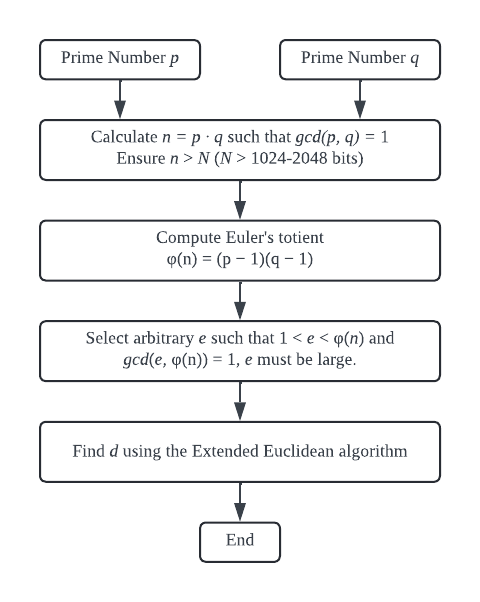
\includegraphics[width=0.5\textwidth]{images/Key Generation.png}
    \caption{RSA Key Generation Procedure}
\end{figure}

\textbf{Euclidean Algorithm}
The Euclidean algorithm provides the basis for finding the modular inverse of $e \mod \phi(n)$ and uses the process of backwards substitution. To find $d$, we apply the extended Euclidean algorithm using the formula
\begin{equation}
\phi(n) = e\cdot q + r
\end{equation}
where $e$ is our public exponent, $q$ is our quotient, and $r$ is our remainder. Just like the general Euclidean algorithm, wherever $r \neq 0$ we repeat the process until we reach $r = 0$. By the method of backwards substitution, we will be able to determine coefficients $x$ and $y$ (Bézout's coefficients), that satisfy the equation $1 = e \cdot x + \phi(n) \cdot y$ where $x$ is our private $d$ exponent. When $d > 0$ we obtain the private key. When $d < 0$ we add the integer $\phi(n)$ to $d$, and this final result will be $d$.

To illustrate this process, we will consider two integers $a$ and $b$, where $b > a$. We denote the relationship between these two integers by
\begin{equation}
b = m_0 \cdot a + r^1
\end{equation}
where when we divide $b$ by $a$, we obtain a multiplier $m_0$, and a remainder $r^1$ such that $gcd(a, b) = gcd(a, r^0)$. Given this relationship, we only need to find the $gcd$ for integers $a$ and $r^0$:
\begin{equation}
\begin{aligned}
b & = m_0 \cdot a + r^1 \\
a & = m_1 \cdot r^1 + r^2 \\
r^1 & = m_2 \cdot r^2 + r^3 \\
&\vdots \\
r^{n-2} & = m_n \cdot  r^{n-1} + r^n
\end{aligned}
\end{equation}
Once the algorithm is complete, the value $r^n = 0$ illustrates that the last non-zero remainder is $gcd(a, b)$. This fact is important in the RSA algorithm as this last non-zero remainder is a core component of the generation of public and private keys used for encryption and decryption.

\subsubsection{Extended Euclidean Algorithm}
The Extended Euclidean algorithm aims to not only find the greatest common divisor, but to determine Bézout's coefficients such that the formula 
\begin{equation}
a \cdot x + n \cdot y = gcd(a, n)
\end{equation}
holds true. We aim to express $gcd(a, n)$ as a linear combination of $a$ and $n$ therefore giving us further insights on the value of private exponent $d$. Employing back substitution, we replace each remainder with its equivalent expression obtained from the previous step in the algorithm until we reach an equation that is entirely expressed as a linear combination of $a$ and $n$, specifically:
\begin{equation}
a \cdot x + n \cdot y = 1
\end{equation}
in the case where $gcd(a,n) = 1$. In this notation, $x$ refers to the private exponent $d$.

\subsubsection{Example: RSA Key Generation}
We will choose two large prime integers, calculate the integer value of Euler's totient function, then apply the Extended Euclidean algorithm to find the modular inverse of $e \mod \phi(n)$. 

\begin{enumerate}
    \item Two large prime integers $p$ and $q$ are chosen.
    
Let $p = 61$, and $q = 53$. We now compute $n$ such that $n = pq$:
\begin{equation}
n = p \cdot q = 61 \cdot 53 = 3233
\end{equation}
\item Compute Euler's Totient Function $\phi(n)$.
Euler's totient function is given by
\begin{equation}
\begin{aligned}
\phi(n) &= (p - 1)(q - 1)\\
&= (61 - 1)(53 - 1)\\
&= 60 \cdot 52\\
&= 3120
\end{aligned}
\end{equation}
We select an arbitrary $e$ that satisfies $1 < e < \phi(n)$ and $gcd(e, \phi(n) = 1$. Typically, the value $65537$ is chosen as it is quite large, however for this example we will proceed with $e = 17$. In selecting our value for $e$, we must confirm that $gcd(17, 3120) = 1$. Since both integers are prime, they satisfy the requirement of being relatively prime such that $e = 17$ is a valid choice. 
\item Compute the modular inverse of $e \mod \phi(n)$.
In this step, we find the value of $d$, which is the modular inverse of $e \mod \phi(n)$ such that
\begin{equation}
e \cdot d \equiv 1 \mod \phi(n)
\end{equation}
We are able to solve this through the Extended Euclidean algorithm method and its process of back substitution. Therefore, we aim to solve the equation
\begin{equation}
17d \equiv 1 \mod(3120)
\end{equation}

\end{enumerate}
We apply the Extended Euclidean algorithm to find the greatest common divisor of $17$ and $3120$:
\begin{equation}
\begin{aligned}
3120 & = 17 \cdot 183 + 9 \\
17 & = 9 \cdot  1 + 8 \\
9 & = 8 \cdot 1 + 1 \\
8 & = 1 \cdot  8 + 0
\end{aligned}
\end{equation}
We have confirmed that $gcd(17, 3120) = 1$, as the last non-zero remainder is 1 as expected given $17$ and $3120$ are relatively prime. We want to express this algorithm in terms of $17$ and $3120$, which is done by back substitution, starting with refactoring our original algorithm:
\begin{equation}
\begin{aligned}
9 &= 3120 - 183 \cdot 17 \\
8 &= 17 - 9 \cdot  1 \\
1 &= 9 - 8 \cdot 1
\end{aligned}
\end{equation}
As we perform our back substitution on values with a remainder, $8 = 8 \cdot 1 + 0$ is removed. First, we substitute $8$ in $9 - 8 \cdot 1 = 1$ with $17 - 9$ given by $8 = 17 - 9$ such that
\begin{equation}
\begin{aligned}
1 &= 9 - 1\cdot(17 - 9)\\
&= 2 \cdot 9 - 1 \cdot 17
\end{aligned}
\end{equation}
We now substitute $9$ in $2 \cdot 9 - 1 \cdot 17$ given by $9 = 3120 - 183 \cdot 17$ such that
\begin{equation}
\begin{aligned}
1 &= 2 \cdot (3120 - 183 \cdot 17) - 1 \cdot 17 \\
&= 2 \cdot 3120 - 367 \cdot 17
\end{aligned}
\end{equation}
As informed by the formula $a \cdot x + n \cdot y = 1$, our $d$ value is $-367$ which is negative. As we know, $d$ must be a positive integer based on the conditions of RSA key generation, we simply add $n$ to $d$ such that
\begin{equation}
-367 + 3120 = 2753
\end{equation}
which is our value for private exponent $d$.

By using the public key $\{17,3233\}$, and private key $\{2753, 3233\}$ we can proceed with the encryption and decryption of our message, $M$.

\subsection{Encryption and Decryption}
\begin{figure}[H]
    \centering
    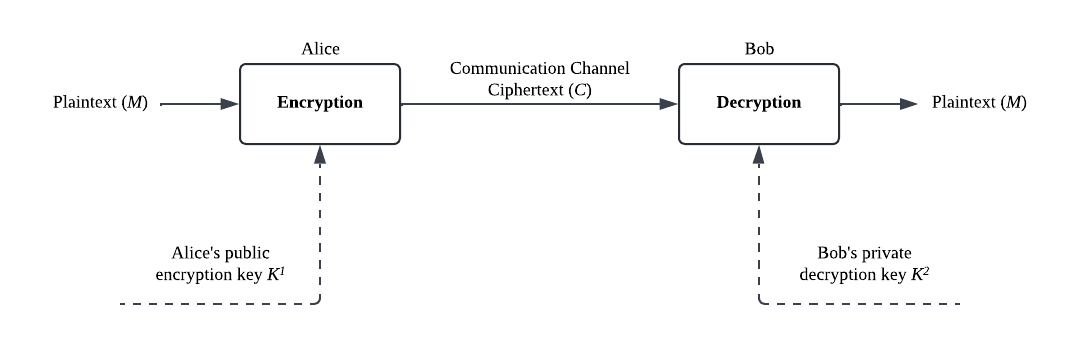
\includegraphics[width=0.9\textwidth]{images/Algorithm Diagram.png}
    \caption{RSA Encryption/Decryption}
\end{figure}
To encrypt a message using the RSA algorithm with a given public encryption key $\{e, n\}$, the general method is outlined as follows:
\begin{enumerate}
    \item We represent the message as an integer value between $0$ and $n-1$, using any standard representation. 
    \item To encrypt the message, we raise it to the $e$th power of $\mod n$ such that the result (ciphertext $C$) is the remainder as informed by $M^e / n$. The encryption procedure can be denoted as the following:
\begin{equation}
C \equiv e(M) \equiv M^e \mod n
\end{equation}
\end{enumerate}
for message $M$.

To decrypt a message, we:
\begin{enumerate}
    \item Raise $M$ to the $d$th power $\mod n$, which is a part of the private key $\{d, n\}$ with the decryption procedure being 
\begin{equation}
M \equiv d(C) \equiv C^d \mod n
\end{equation}
for ciphertext $C$.
\end{enumerate}

\subsubsection{Example: Encryption and Decryption Using RSA}
Given the values $e = 17$, $d = 2753$, and $n = 3233$ from the previous key generation example, we will encrypt a message $M = 123$ in the following steps:
\begin{enumerate}
    \item Input all relevant values into the encryption formula:
\begin{equation}
\begin{aligned}
C &= M^e \mod n\\ 
&= 123^{17} \mod 3233
\end{aligned}
\end{equation}
\item Calculate for ciphertext $C$:
\begin{equation}
\begin{aligned}
C &= 123^{17} \mod 3233\\ 
&= 855
\end{aligned}
\end{equation}
\end{enumerate}
We will now decrypt the ciphertext $C$, given we have obtained the private exponent $d$ within the private key $\{d, n\}$ we can solve the decryption formula:
\begin{equation}
\begin{aligned}
M &= C^d \mod n\\
&= 855^{2753} \mod 3233\\
&= 123
\end{aligned}
\end{equation}
This completes the example for encryption and decryption using the RSA Algorithm.

\section{Correctness of the RSA Algorithm}
We aim to illustrate the proof behind the RSA Algorithm where we show that we are able to recover the value of $M$ after decryption and that the decryption procedure works \cite{sridharan}. 

\begin{proof}
Illustrating the correctness of the algorithm, we begin with this key identity from Euler's theorem:
\begin{equation}
M^{\phi(n)} \equiv 1 \mod n
\end{equation}
where $M$ is relatively prime to $n$ ($gcd(M, n) = 1$) and $\phi(n)$ is Euler's totient function, which provides the number of integers between $1$ and $n$ that are relatively prime to $n$. For a prime number $p$, we have:
\begin{equation}
    \phi(p) = p-1
\end{equation}
This can then be applied to another prime $q$ to show that:
\begin{equation}
\begin{aligned}
    \phi(n) &= \phi(p)\cdot \phi(q)\\
    &= (p-1)(q-1)\\
\end{aligned}
\end{equation}
Given $e$ and $d$ are chosen such that $d$ is the multiplicative inverse of $e \mod \phi(n)$:
\begin{equation}
e \cdot d \equiv 1 \mod \phi(n)
\end{equation}
We are now able to prove that encryption and decryption are in fact reverse operations by observing encryption function $E(M) = M^e \mod n$ and decryption function $D(C) = C^d \mod n$ such that we derive the following:
\begin{equation}
   D(E(M))\equiv (M^e)^d \equiv (M)^{e\cdot d} \mod n\\
\end{equation}
Since we know that $e \cdot d = 1 \mod \phi(n)$, we can state that
\begin{equation}
M^{e \cdot d} \equiv M^{k \cdot \phi(n)+1} \mod n
\end{equation}
for some integer $k$. Since we know that $gcd(M, p) = 1$, Euler's theorem gives us
\begin{equation}
M^{p-1} \equiv 1 \mod p
\end{equation}
which follows that
\begin{equation}
M^{k\phi(n)+ 1} \equiv M \mod p
\end{equation}
Similarly, since $gcd(M, q) = 1$:
\begin{equation}
M^{k\phi(n)+ 1} \equiv M \mod q
\end{equation}
and by Euler's theorem $M^{k \phi(n)} \equiv 1$, so we can show that
\begin{equation}
M^{k\phi(n)+ 1} \equiv M \mod n
\end{equation}
Therefore, we arrived at our desired result:
\begin{equation}
M^{e\cdot d} \equiv M \mod n
\end{equation}
which demonstrates that $e$ and $d$ are inverse permutations, completing the proof. 
\end{proof}

\subsection{Efficiency Discussions}
Successive squaring is an algorithmic technique that is used to calculate exponentiation at a high speed whilst reducing the amount of multiplications required to do so. Applying this technique allows modular arithmetic and cryptographic operations to become much more efficient thus enhancing the protection of information. 

\subsubsection{Application of Successive Squaring}
In the RSA algorithm, we raise a message $M$ to the power of $e$, or $d \mod n$, where $n$ is the product of two large prime integers. Whilst we can directly compute the formulas $M^e \mod n$ and $C^e \mod n$ (with $C$ being the ciphertext), it can prove difficult when $e$ and $d$ are absurdly large integers. It makes more sense to employ an algorithm to handle these in a more efficient manner. Rather than calculating the exponentiation in a straightforward way, successive squaring utilises squaring alongside multiplication based on the binary expansion of the exponent, resulting in a reduction in the number of operations required \cite{successive}. In this application, our aim is to solve the equation $M^e \mod n$ represents the process of encrypting our message $M$.

Suppose we want to solve $5^{196} \mod 28$ where we begin by creating a table which gives us the values of 5, $5^2$, $5^4$, $5^8$, and so on until we reach a power that is just below $e$. For each successive entry in the list, we simply have to square the number in the $M^e$ position of the result this meaning we never work with integers above our $e$ exponent. The table will look like this:

\begin{table}[H]
    \centering
    \begin{tabular}{ccccccccc}
         $5^1$&  $\equiv$&  $5^1$&  $\equiv$&  $5$&  $\equiv$&  $5$&  $\equiv$& $5 \mod 28$\\
         $5^2$&  $\equiv$&  $(5^1)^2$&  $\equiv$&  $25$&  $\equiv$&  $25$&  $\equiv$& $25 \mod 28$\\
         $5^4$&  $\equiv$&  $(5^2)^2$&  $\equiv$&  $25^2$&  $\equiv$&  $625$&  $\equiv$& $9 \mod 28$\\
         $5^8$&  $\equiv$&  $(5^4)^2$&  $\equiv$&  $9^2$&  $\equiv$&  $81$&  $\equiv$& $25 \mod 28$\\
         $5^{16}$&  $\equiv$&  $(5^8)^2$&  $\equiv$&  $25^2$&  $\equiv$&  $625$&  $\equiv$& $9 \mod 28$\\
         $5^{32}$&  $\equiv$&  $(5^{16})^2$&  $\equiv$&  $9^2$&  $\equiv$&  $81$&  $\equiv$& $25 \mod 28$\\
         $5^{64}$&  $\equiv$&  $(5^{32})^2$&  $\equiv$&  $25^2$&  $\equiv$&  $625$&  $\equiv$& $9 \mod 28$\\
         $5^{128}$&  $\equiv$&  $(5^{64})^2$&  $\equiv$&  $9^2$&  $\equiv$&  $81$&  $\equiv$& $25 \mod 28$\\
    \end{tabular}
    \caption{Successive Squaring: $5^{196} \mod 28$}
\end{table}

We then proceed with the binary expansion $196$ which is $11000100$. In visualising our binary expansion like the following:

\begin{table}[H]
    \centering
    \begin{tabular}{cccccccc}
         $5^1$&  $5^2$&  $5^4$&  $5^8$&  $5^{16}$&  $5^{32}$&  $5^{64}$& $5^{128}$\\
         $5$&  $25$&  $9$&  $25$&  $9$&  $25$&  $9$& $25$\\
         $0$&  $0$&  $1$&  $0$&  $0$&  $0$&  $1$& $1$\\
    \end{tabular}
    \caption{Binary Expansion: 196}
\end{table}
we can see the $1$'s align with $5^{128}$, $5^{64}$, and $5^{4}$ which when added:
\begin{equation}
\begin{aligned}
    5^{128+64+4} & = (5^{128})(5^{64})(5^4)\\
    &= (25)(9)(9)\\
    &= 2025\mod 28\\
    &= 9\mod 28\\
    \end{aligned}
\end{equation}
gives the solution to the equation $5^{196} \mod 28$.

The following are the general steps to solve equations in the form $a^k \mod n$ utilising the method of successive squaring:
\begin{enumerate}
    \item Write $k$ as a sum of powers of $2$:
\begin{equation}
    k = u_0 + u_1 \cdot 2 + u_2 \cdot 4 + u_3 \cdot 8+ \ldots + u_r \cdot 2^r
\end{equation}
where each $u_i$ can be expressed in their binary representation ($1$ or $0$). 
\item Create a table of powers of $a \mod n$ and begin the successive squaring technique to populate the table.
\begin{table}
    \centering
    \begin{tabular}{ccccccc}
         $a^1$&  $\equiv$&  &  $\equiv$&  &  $\equiv$& $A_0 \mod n$\\
         $a^2$&  $\equiv$&  $(a^1)^2$&  $\equiv$&  $A^2_0$&  $\equiv$& $A_1 \mod n$\\
         $a^4$&  $\equiv$&  $(a^2)^2$&  $\equiv$&  $A^2_1$&  $\equiv$& $A_2 \mod n$\\
         $a^8$&  $\equiv$&  $(a^4)^2$&  $\equiv$&  $A^2_2$&  $\equiv$& $A_3 \mod n$\\
         &  $\vdots$&  &  $\equiv$&  &  & $\vdots$\\
         $a^{2^r}$&  $\equiv$&  $(a^{2^{r-1}})^2$&  $\equiv$&  $A^2_{r-1}$&  $\equiv$& $A_r \mod n$\\
    \end{tabular}
    \caption{Successive Squaring: Notation}
\end{table}
\item The product as a result of this successive squaring is:
\begin{equation}
 A^{u_0}_0 \cdot A^{u_1}_1 \cdot A^{u_2}_2 \ldots A^{u_r}_r  \mod n 
\end{equation}
\item Examine the binary representation of $a^k$ and identify which indices $i$ correspond to $u_i = 1$. To get the final result, we multiply the corresponding $A_i$ terms:
\end{enumerate}
\begin{equation}
    a^k \mod n = \prod_{i=0}^{r} A_i^{u_i} \mod n
\end{equation}
where $A_i$ corresponds to $u_i$ for each $i = 1$.  This approach aims to utilise the binary expansion of $k$ to determine exactly which values of $a \mod n$ should be included in the final multiplication to return the desired result. 

\section{Modern Applications of RSA}
Although revolutionary, the Diffie-Hellman algorithm was notably insecure due to its lack of appropriate verification methods. Rivest, Shamir, and Adleman's new cryptosystem proposal aimed to introduce a more secure avenue for enciphering and deciphering data transmission over the Internet. As the Internet grew in popularity, the demand for better security grew in parallel, especially in areas such as banking and electronic mail. Users value secrecy and the protection of their sensitive information, so there must have been a way to prevent others from accessing this information. The RSA algorithm was unique in its implementation of a private key {$d, e$} in which only the authorised receiver could use. From this application, the RSA algorithm is observed in many different forms, from SSL and TLS protocols to digital signatures and email encryption software such as PGP (Pretty Good Privacy), and GPG (Gnu Privacy Guard). As your average person has very little understanding of how these encryption algorithms work, they may not even know how often they are utilised, let alone how powerful they can be for data protection. 

\subsubsection{Transport Layer Security Protocols}
Transport Layer Security (TLS) is a protocol that secures digital communication on the Internet. RSA is among the two most common choices for TLS certificates \cite{ssl}. RSA's role in this exchange is to facilitate secure communication between an end-user and a server. In a TLS handshake procedure, a user connects to a website (typically via HTTPS), and the server will then send its TLS certification which contains its public key, to the end-user. This certificate is cross-checked against Certified Authorities (CAs) to confirm the server's identity. The user then generates a pre-master secret which is encrypted utilising the public key from the TLS certificate. When the server receives this pre-master secret, it is able to decrypt it using its private key, deriving the symmetric keys from within the pre-master secret. Thus, a secure communication channel is then established between the user and the server.

\begin{figure}[ht]
    \centering
    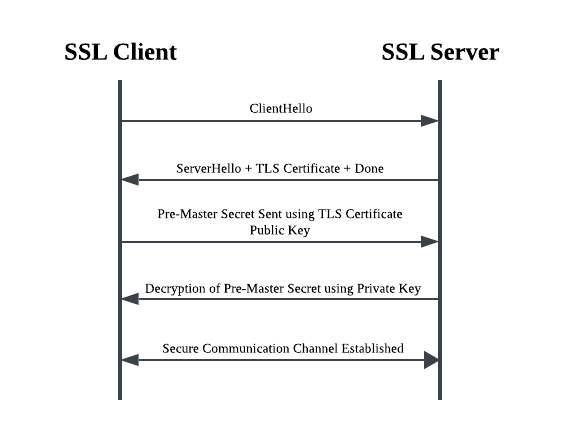
\includegraphics[width=0.7\textwidth]{images/TLS Diagram.png}
    \caption{TLS Handshake Process}
\end{figure}

\subsubsection{Digital Signatures}
In the modern digital age, verifying the authenticity and integrity of a message has never been more important. RSA is often used to generate and verify digital signatures where a message is hashed using a hash function, which is then encrypted using the user's private key to construct the digital signature ensuring that the identity of the sender is embedded in the data transmission. The recipient of the message then uses the sender's public key to decrypt the signature and then subsequently compares this result to a hash of the received message, thus verifying the users identity and the authenticity of the communication.

\subsubsection{Email Encryption}
Through tools like Pretty Good Privacy (PGP) and Gnu Privacy Guard (GPG) the RSA algorithm is utilised in order to ensure confidentiality and authenticity of electronic mail transmission. It's application in both PGP and GPG is quite similar to our general exploration of the algorithm such that the sender encrypts the message with their public key $e$, and the receiver decrypts the message with their private key $d$. PGP and GPG also allow communications to be digitally signed to ensure the authenticity and integrity of the communication. 

Departing from these more preliminary applications of the RSA algorithm, modern systems continue to implement the algorithm to ensure security of user data. Online banking and financial transaction services adopt the use of RSA given the sensitive nature of these types of operations, particularly when dealing with actual currency. Suppose a user logs into their banking application, the RSA algorithm ensures that the user has the ability to exchange their credentials securely. In this interaction, the user's browser generates a session key which is then encrypted utilising the bank's private key which ensures that any authentication tokens or account information is protected under the algorithm. This principle is similarly applied to secure financial transactions, VPN communications, and even e-Commerce websites in which secure information must be protected from 'Man-in-the-Middle' attacks. 

\subsection{Factoring Large Integers in RSA}
RSA is constructed on the basis that, whilst it is easy to multiply two numbers $p$ and $q$ to produce a large composite number $n$, it is not so easy to reverse this process, especially when the size of these prime numbers increases exponentially. Knowledge of the prime factors of $p$ and $q$ is key in obtaining the private exponent $d$, such that if an attacker is able to factor $n$ they will be successful in obtaining the private key $d$; therefore breaking the encryption. This very asymmetry of complexity is what made the RSA algorithm such a vast improvement over the Diffie-Hellman algorithm. 

There is currently no known algorithm that has the ability to factor large numbers in an acceptable time, such that even for a number of $1024$ bits it may take years or decades to factor. However, the looming threat of quantum computing serves to challenge this idea. Quantum computers are known for their ability to perform multiple algorithms in a single step, making the solution to particular mathematic problems more efficient. One problem is factoring large numbers, which is crucial in maintaining the security of the RSA algorithm. 

\subsubsection{Shor's Algorithm: The Biggest Threat}
Shor's algorithm \cite{shor}, named after its creator Peter Shor, is a quantum algorithm that was introduced in $2001$, and it provides a way to efficiently factor large composite numbers by utilising polynomial time, a time complexity which is impossible for classical computers, as they rely purely on exponential-time algorithms. Suppose we were able to find a large-scale quantum computer running Shor's algorithm, this computer could theoretically break the RSA algorithm due to its power.
 
\subsection{Vulnerabilities in RSA Cryptography}
"Twenty Years of Attacks on the RSA Cryptosystem" penned by Dan Boneh \cite{attacks} outlines four categories of RSA attacks:
\begin{itemize}
    \item Elementary Attacks 
    \item Low Private Exponent 
    \item Low Public Exponent, and
    \item Implementation Attacks 
\end{itemize}
where given the advancement of technology have become increasingly common on the algorithm.

\subsubsection{Elementary Attacks}
These types of attacks demonstrate an overt misuse of the RSA cryptosystem. One such example is if multiple users share the exact same $\mod n$ as although both users have a unique private key pair $\{e_i, d_i\}$) it is possible that ciphertexts intended for one user Alice, can be decrypted by another user, Bob thus meaning he is able to derive Alice's private key by using his own key pair thus allowing him to factor $C$. This establishes the importance of ensuring that no RSA modulus should be used by more than one user. 

Let's say Alice and Bob are both provided with the same modulus $n = p\cdot q$ and each user has their own pair of public and private keys denoted as the following: 
\begin{itemize}
    \item Alice has a public key $\{n, e_a\}$, a private key $d_a$, where $e_a \cdot d_a \equiv 1 \mod \phi(n)$
    \item   Bob has a public key $\{n, e_b\}$, a private key $d_b$, where $e_b \cdot d_b \equiv 1 \mod \phi(n)$
\end{itemize}
Suppose that after Alice has enciphered her message and sends it through to someone using her public key $e_A$ and her $\mod n$ , Bob wishes to decrypt the message. While it is true that Bob will not be able to directly decipher Alice's message $C^A$, he can attempt to factor modulus $n$. As Bob has access to $\{n, d_B, e_B\}$ he is able able to derive $\phi(n)$ by computing
\begin{equation}
    e_B \cdot d_B \equiv 1 \mod \phi(n)
\end{equation}
With $\phi(n)$, Bob will now be able to obtain Alice's private key $d_A$ by utilising her public key in the formula
\begin{equation}
    e_A \cdot d_A \equiv 1 \mod \phi(n)
\end{equation}
and Bob has now successfully extracted Alice's private key $d_A$. 

\subsubsection{Low Private Exponent}
Whilst using a small private key $d$ greatly improves the speed of decryption or signature generation, it is possible that if $d$ is too small, there is a way to derive this private key from $n$ and $e$ should $d$ be fewer than $256$ bits in length. This is observed in Weiner's \cite{attacks} attack, where, with a small private key $d$ (explicitly when it is smaller than $1/3^{n^{1/4}}$, where $n$ is the modulus) a potential attacker has the ability to compromise the encryption by recovering $d$ through mathematical methods such as continued fractions, devastating the security of RSA. Thus, it is implored to choose a large public key $e$ to prevent this type of breach.

\subsubsection{Low Public Exponent}
Similarly to utilising a small private key, a small public key $e$ can also compromise the security of the RSA algorithm and expose a system to attacks such as Håstad's Broadcast Attack, or Partial Key Exposure Attack \cite{attacks}, should $e$ be too small. Such attacks exploit the mathematical properties of encryption when $e$ is too small, leading to attackers being able to encipher messages they are unauthorised to see. Thus, selecting a large exponent $e$, whilst increasing computational time is a far safer and more secure option then selecting a small public exponent.

\subsubsection{Implementation Attacks}
Implementation attacks explore circumstances in which the implementation of the RSA algorithm is exploited. 'Timing' attacks are one such attack which exploits this very aspect as it relies on calculating the time it takes to perform the decryption alongside details about the system itself to determine the value of $d$. 

To aid in illustrating this type of attack, suppose a smartcard which stores a private RSA key is created to be tamper-resistant such that Marvin is unable to directly access the private key inside. It was discovered by Kosher that if Marvin was able to measure the time it took to perform RSA decryption or signing, private key $d$ could be obtained. Decryption is typically performed through successive squaring such that $C = M^d \mod n$ is computed and its binary expansion $a = a_d, a_{d-1}, a_{d-2}, \ldots a_0$ where $a_i \in$ $\{1,0\}$

We first initialise $z$ to $M$ and $C$ to $1$ and then for each bit $a_i$ of $a$ from the least to the most significant, if $a_i = 1$, $C$ is updated to $(C\cdot z) \mod n$. $z$ is subsequently updated to $z^2 \mod n$.  The multiplication operation $C \cdot z$ is performed when Marvin sends random messages and measures the time it takes ($T_i$) to compute $C_i = M{^{d_i}} \mod n$, allowing him to determine whether $d_1$ is 1 or 0. This method provides Marvin with enough information to obtain the private key $d$ based on its binary representation. 

\section{Conclusion}
In this paper, we have explored the RSA algorithm and its mathematical properties which ensure its security even in modern implementations. We have observed that RSA is fundamentally a straightforward piece of mathematics, which utilises the facts and theorems of other mathematical concepts such as number theory, modular exponentiation, and Euler's theorem. We have successfully illustrated the correctness of the RSA algorithm through testing, including both key generation and decryption processes. Our results substantiate that a message encrypted with a public key can be subsequently decrypted with the corresponding private key. This proof demonstrates the algorithm's effectiveness as well as its ability to preserve secure data transmission. In understanding these proofs and their applications, we lay the foundation for further exploration of cryptographic algorithms and open conversations for evaluating the future of these types of systems when faced with threats such as quantum computing. RSA has had an influential impact on encryption algorithms since its proposal in $1977$, and understanding the mathematical principles that make up the algorithm enhances one's appreciation for its significance and influence in modern day systems, such as for secure transaction processes, and supporting SSL/TLS protocols. Cryptography, much like technology in general, is progressing exponentially, with new advancements in technology being introduced all the time. With these advancements comes technology that poses a significant threat to the security of algorithms like RSA such as quantum computing. The direction of future research must focus on advancing quantum-resistant algorithms to better protect data transmission against potential attackers. Alternatives such as lattice-based cryptography \cite{lattice}, and hash-based functions alongside other innovative frameworks must be considered. By remaining proactive in our approach to maintaining the integrity of data through emerging technologies, we ensure the security of digital communications for future generations. 

\clearpage
\begin{thebibliography}{9}
\bibitem{rsa1977} R. L. Rivest, A. Shamir, and L. Adleman, “A method for obtaining digital signatures and public-key cryptosystems,” Communications of the ACM, vol. 21, pp. 120–126, 1978. doi: \url{https://doi.org/10.1145/359340.359342}.

\bibitem{DH} W. Diffie and M. Hellman, “New directions in cryptography,” IEEE Transactions on Information Theory, vol. 22, pp. 644–654, 1976. doi: \url{https://doi.org/10.1109/tit.1976.1055638}.

\bibitem{eulerstheorem} K. Conrad, “Euler’s theorem,” 2015. [Online]. Available: \url{https://kconrad.math.uconn.edu/blurbs/ugradnumthy/eulerthm.pdf}.

\bibitem{keygeneration} A. Grami, “Cryptography,” Discrete Mathematics, pp. 197–210, 2023, doi: \url{https://doi.org/10.1016/b978-0-12-820656-0.00011-3}.

\bibitem{sridharan} S. Sridharan and R. Balakrishnan, Discrete Mathematics, CRC Press, pp.259, 2019.

\bibitem{successive} Adkins. M, “Powers via Successive Squaring.” 2009. [Online]. Available: \url{https://www.math.lsu.edu/\~adkins/m4023/SuccessivePowers.pdf}.

\bibitem{ssl} P. Nohe, “Taking a Closer Look at the SSL Handshake,” 2019. [Online]. Available: \url{https://www.thesslstore.com/blog/explaining-ssl-handshake/‌}‌

\bibitem{shor} P. W. Shor, “Polynomial-Time Algorithms for Prime Factorization and Discrete Logarithms on a Quantum Computer,” SIAM Journal on Computing, vol. 26, no. 5, pp. 1484–1509, 1997. 
\url{doi: https://doi.org/10.1137/s0097539795293172}.

\bibitem{attacks} D. Boneh, “Twenty years of attacks on the RSA cryptosystem. Notices of the AMS”, vol. 46(2), pp. 203–213, 1999.

\bibitem{lattice} D. Micciancio and O. Regev, “Lattice-based Cryptography,” Post-Quantum Cryptography, pp. 147–191, 2009, doi: \url{https://doi.org/10.1007/978-3-540-88702-7\_5}.
\end{thebibliography}
\end{document}
